\section{System Architecture}

\subsection{Architecture Overview}
RollupX is designed as a modular, decoupled Layer-2 (L2) benchmarking sandbox. As illustrated in Fig.~\ref{fig:architecture}, it separates the rollup lifecycle into isolated stages: workload generation, transaction sequencing, execution, zero-knowledge proving, and L1 submission. This isolation allows individual protocol parameters (e.g., batch size, timeouts, ordering policies, and data availability modes) to be modified independently without confounding variables from other layers.

\begin{figure}[h]
    \centering
    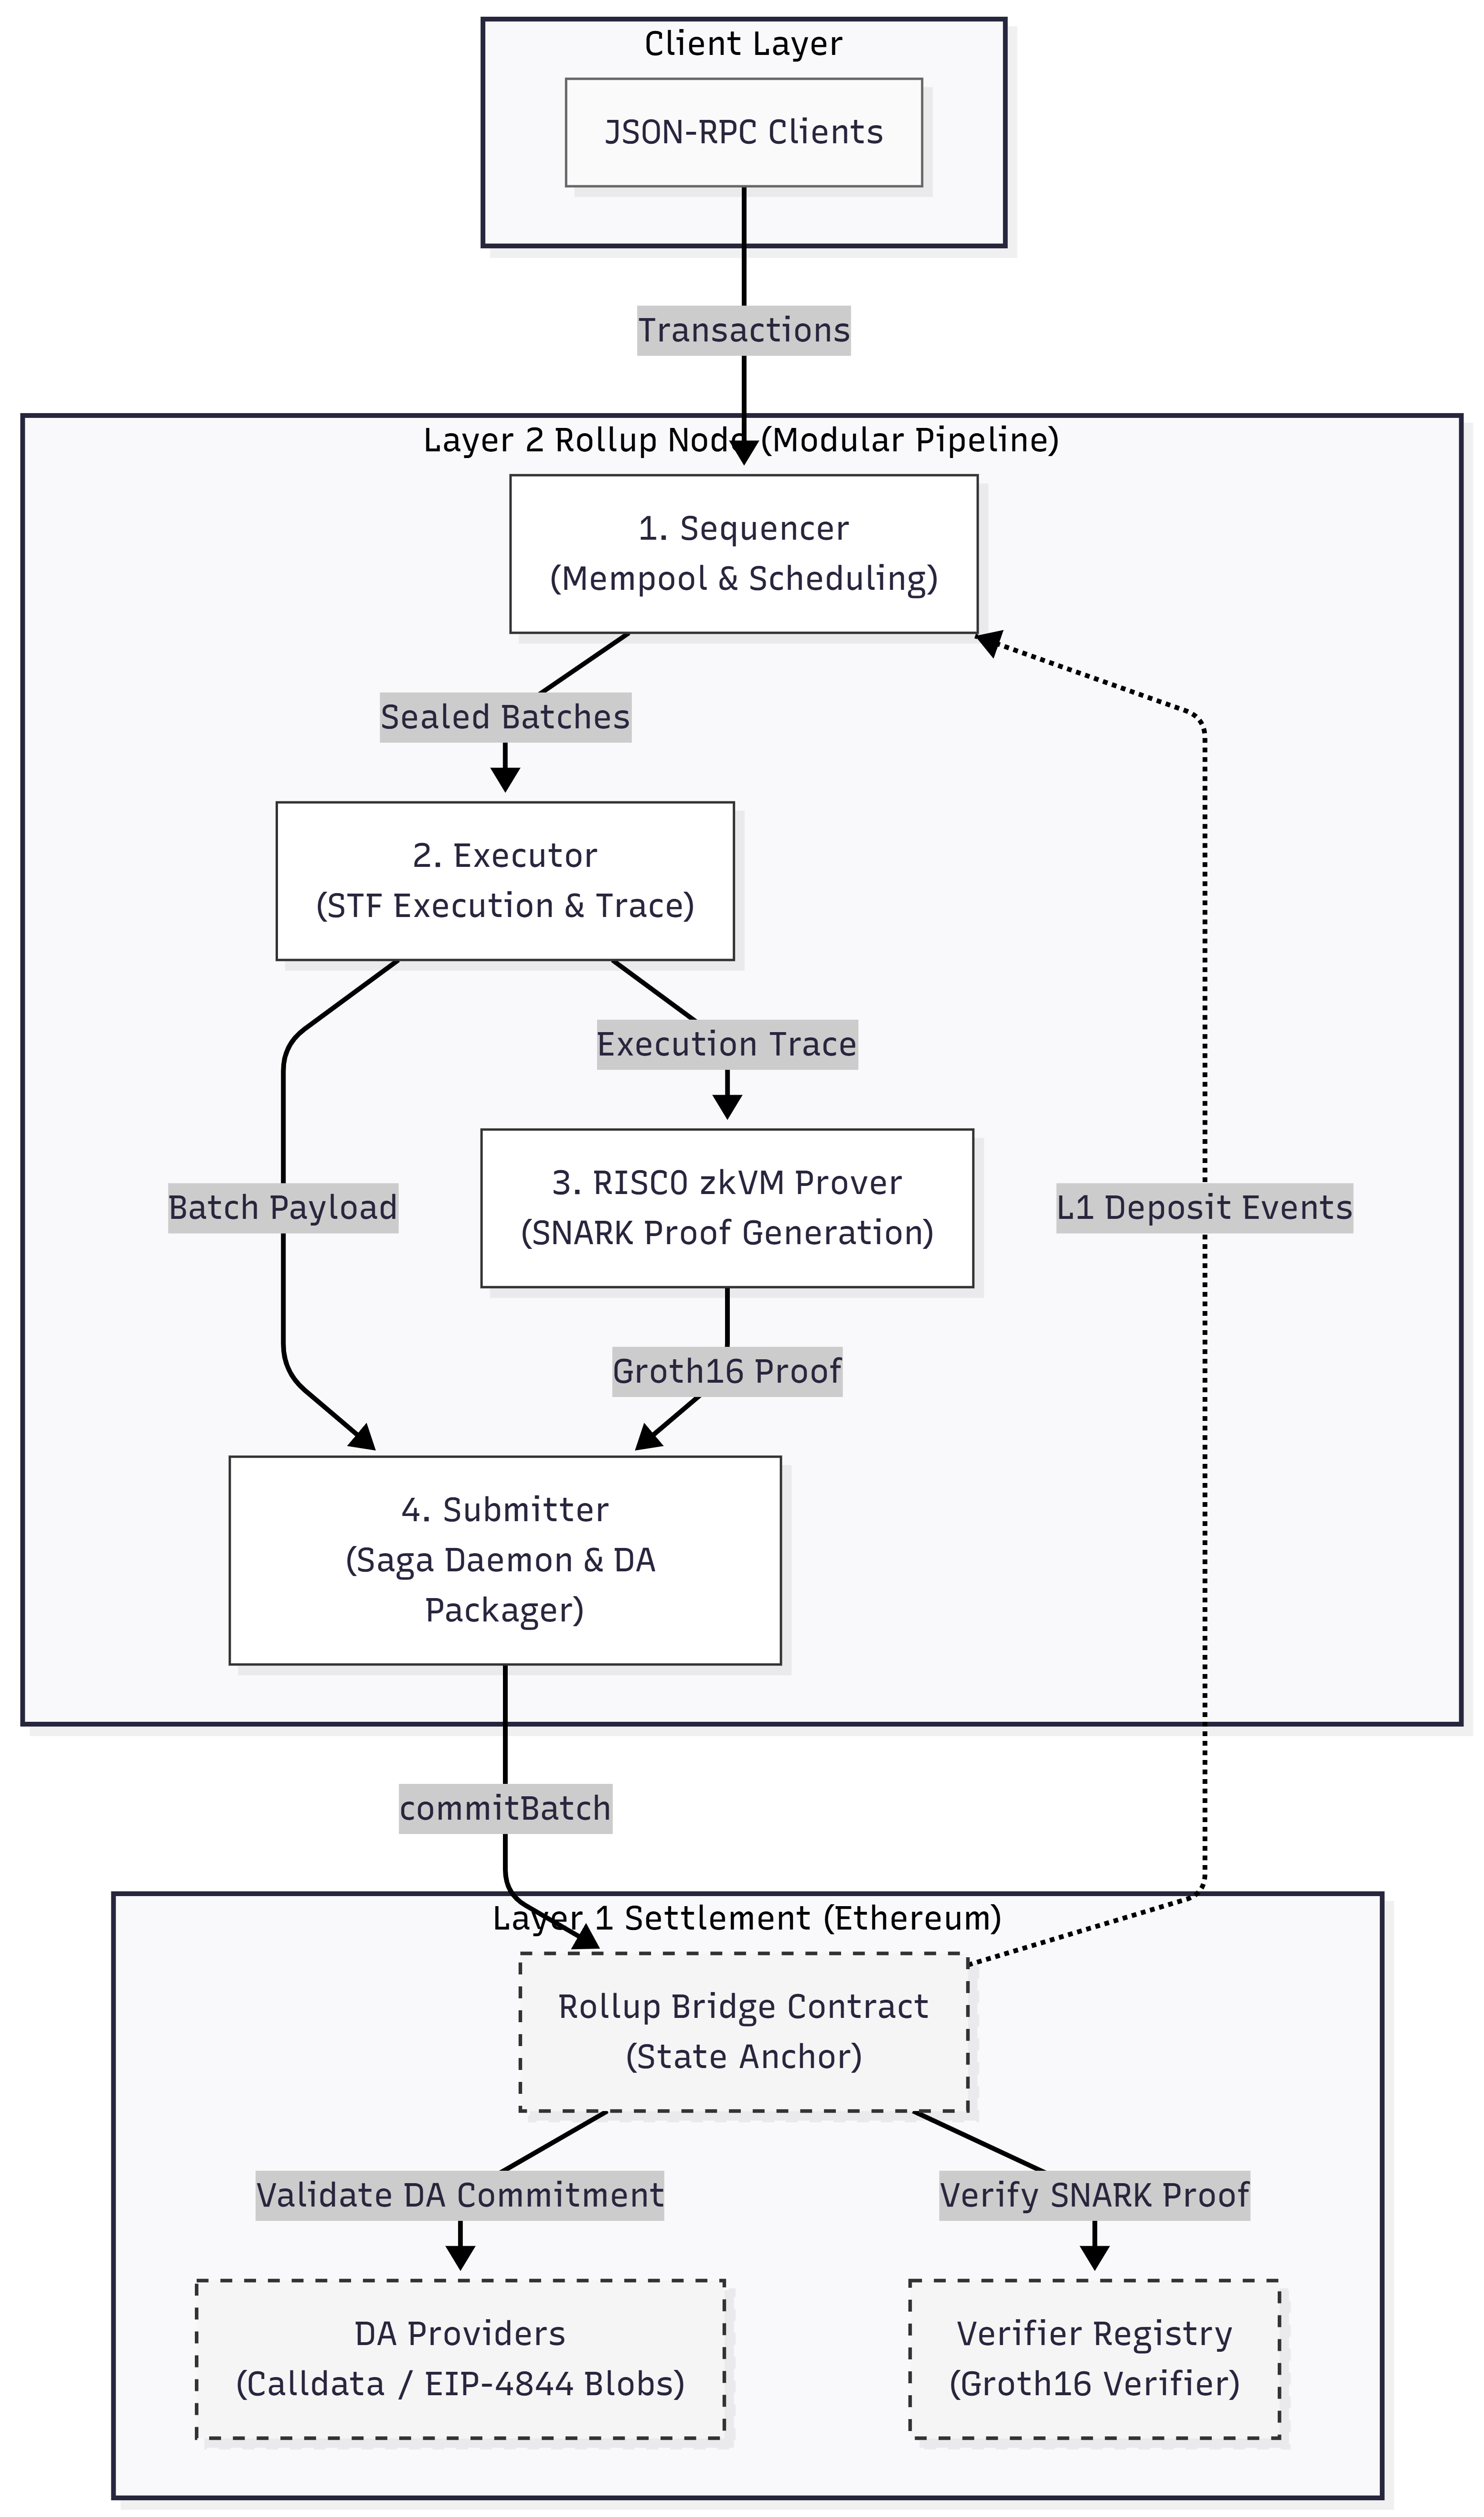
\includegraphics[width=1\linewidth]{system architecture.png}
    \caption{RollupX modular prototype system architecture diagram.}
    \label{fig:architecture}
\end{figure}

\subsection{Core Components}
The prototype is structured into seven modular components:
\begin{itemize}
    \item \textbf{Workload Generator \& Ingestion:} Generates transaction workloads of Poisson or bursty nature and validates the ingestion of those transactions through a HTTP JSON-RPC endpoint.
    \item \textbf{Sequencer:} Manages the mempool, orders incoming transactions using configured scheduling policies (e.g., FCFS, TimeBoost), and groups them into sealed batches when size limits or timeouts are met.
    \item \textbf{Executor:} Consumes batches of sealed data and runs the state transition function to process the transactions within those batches and commit the new states of the L2 accounts to the Sparse Merkle Tree.
    \item \textbf{Prover (RISC0):} Runs the state transition function within the RISC0 zkVM, validates the transactions, and commits a STARK proof of validity that is compressed into a 256-byte Groth16 proof.
    \item \textbf{DA Handler \& Submitter:} Takes the batch data and proof, packages them into calldata or Ethereum blobs, and commits them to the L1 blockchain via the commitBatch transaction..
    \item \textbf{L1 verifier contracts:} Deployed on Hardhat, \texttt{RollupBridge.sol} anchors the L2 state root and manages funds, while \texttt{Groth16Verifier.sol} verifies the validity proofs.
    \item \textbf{Telemetry Harness:} Collects execution logs and timestamps across all stages to measure throughput, queue wait times, proving cycles, L1 gas usage, and latency.
\end{itemize}

\subsection{Component-Level Architecture}

The following subsections detail the internal design of each of the components depicted in Fig. 1. Each of the components is implemented in Rust and communicates with other components through well-defined interfaces (either gRPC streams or in-process channels), allowing for each of the components to be individually replaced without impacting the rest of the system.

\subsubsection{Sequencer}

\begin{figure}[h]
    \centering
    \includegraphics[width=1\linewidth]{sequencer.png}
    \caption{Internal architecture of the Sequencer component.}
    \label{fig:sequencer}
\end{figure}

The Sequencer, shown in Fig.~\ref{fig:sequencer}, is the entry point for all transactions submitted by users to the Layer 2 blockchain. The Sequencer receives JSON-RPC requests that contain transactions from users to be validated. These transactions are immediately sent to a Validity Checker to ensure that the transactions are valid (e.g., have a valid signature, appropriate nonce, and sufficient balance). Valid transactions are sent to the normal Transaction Pool, while transactions determined to be deposits or forced exits are sent to the Forced Transaction Queue, which is guaranteed to be included into the next batch of transactions submitted to the Layer 2 blockchain prior to any transactions that are present in the normal Transaction Pool.

Batch formation is governed by a configurable \textit{Batch Engine} that fires when either a maximum transaction count or a wall-clock timeout is reached. Before sealing, the \textit{Scheduler Policy Engine} imposes the active ordering policy such as FCFS, Fee-Priority, Time-Boost, or Fair-BFT over the normal pool, always prepending forced transactions. The resulting ordered sequence is sealed and its metadata (batch ID, transaction count, timestamp) written to a \textit{Batch Registry}, after which the sealed batch is forwarded to the Executor via gRPC. Soft confirmations are returned to the originating client without waiting for L1 settlement.

\subsubsection{Executor}

\begin{figure}[h]
    \centering
    
\includegraphics[width=1\linewidth]{executor.png}
    \caption{Internal architecture of the Executor component.}
    \label{fig:executor}
\end{figure}
The Executor, shown in Fig.~\ref{fig:executor}, takes sealed batches from the Sequencer over a gRPC stream. The main module of the Executor, \texttt{service.rs}, orchestrates the work of four sub-modules.

The \textit{Transaction Engine}, implemented as \texttt{tx\_engine.rs}, takes a transaction, normalizes it, and applies the State Transition Function (STF). The resulting state diffs are written to the RocksDB-backed \textit{State Manager} (\texttt{state.rs}), which maintains the authoritative Sparse Merkle Tree (SMT) and returns the updated state root.

The \textit{Trace Persistence} module (\texttt{trace.rs}) records a deterministic \texttt{BlockTrace} structure together with its hash for subsequent proof verification.

The \textit{Prover Backend Integration} module (\texttt{proof.rs}) invokes the RISC Zero host prover, passing the block trace as input and receiving a SNARK proof and journal as output.

Finally, the \textit{Block Constructor} (\texttt{block\_constructor.rs}) assembles an enriched batch payload containing the state root, proof, and trace metadata, and streams it to the Submitter.

\subsubsection{Prover}

\begin{figure}[h]
    \centering
    
\includegraphics[width=1\linewidth]{prover.png}
    \caption{Internal architecture of the RISC0 Prover component.}
    \label{fig:prover}
\end{figure}

The Prover, shown in Fig. 4, implements a two-tiered architecture that first generates a STARK proof and then produces a Groth16 proof of that STARK proof. The Executor invokes the Host Prover Binary (host/main.rs), passing it the serialised BlockTrace.json file. The Host Prover Binary sends the trace to the RISC0 zkVM through its input channel, where the ZK Circuit Guest (guest/main.rs) executes. Within the guest, calls are made into the rollup core library to apply each state diff to the SMT verifier, to compute the new state root, and to assert that the root matches the one computed by the Executor. If the assertion passes, the guest commits a public journal containing the root and metadata, after which control returns to the host. The host generates a Groth16 proof of the receipt generated by the RISC0 zkVM, producing a constant-size 256-byte proof artifact. The proof, journal, and metadata is returned to the Executor. Additionally, the Executor may also verify the hashes of these artifacts before sending them downstream

\subsubsection{Submitter}

\begin{figure}[h]
    \centering
    
\includegraphics[width=1\linewidth]{submitter.png}
    \caption{Internal architecture of the Submitter (DA Handler) component.}
    \label{fig:submitter}
\end{figure}

The Submitter, shown in Fig.~\ref{fig:submitter}, is a daemon that consumes batch payloads enriched with execution metadata from the Executor via a GrpcBatchSource. An Application Orchestrator implements the saga-style control flow for batches. Upon receiving a batch from the Executor, the Application Orchestrator transitions the batch to the Discovered state, persists the batch to a StorageAdapter (using both SQLite and Postgres databases), and selects a DA strategy for the batch: either calldata encoding or EIP-4844 blob encoding. The chosen \textit{DA Strategy} module formats and encodes the payload, and hands it to an \texttt{L1Connector} built on \texttt{ethers-rs}, which broadcasts the \texttt{commitBatch} transaction to the Ethereum L1 RPC node. The orchestrator then polls for on-chain confirmation; once the transaction is finalised, the batch state is updated to \textit{Confirmed} (or \textit{Failed}) and the record is persisted, completing the saga.

\subsubsection{L1 Smart Contracts}

\begin{figure}[h]
    \centering
    
\includegraphics[width=1\linewidth]{hardhat.png}
    \caption{L1 smart contract architecture deployed on the Hardhat local testnet.}
    \label{fig:l1contracts}
\end{figure}

The on-chain layer, represented in Fig.~\ref{fig:l1contracts}, is deployed on the Hardhat local testnet and consists of two contracts. The main contract, named \texttt{ZKRollupBridge.sol}, receives calls of \texttt{commitBatch} from the Submitter. It delegates the task of validating data availability to the current implementation of the DA Provider (\texttt{CalldataDA}, \texttt{BlobDA}, or \texttt{OffChainDA}), each implementing the \texttt{IDAProvider} interface. Additionally, it delegates the verification of the ZK proofs to the current implementation of the ZK Proof Verifier. Implementations include \texttt{Groth16Verifier}, \texttt{Plonky2Verifier}, and \texttt{MockVerifier}, used in the experiment groups that do not include the proving step. Each of these components uses interfaces to allow for easy swapping of the DA Provider or the ZK Proof Verifier by simply redeploying the implementation contract of the desired component.

\subsection{Design Decisions}
To support controlled benchmarking, RollupX implements the following design decisions contrasting with state-of-the-art (SOTA) production architectures:
\begin{itemize}
    \item \textbf{Execution Engine (Simplified vs.\ zkEVM):} Currently, the leading systems deploy zkEVMs that compile and execute the Ethereum Virtual Machine (EVM) bytecode \cite{scroll_docs}. RollupX employs a simpler, transfer-only execution engine whose State Transition Function (STF) is compiled directly from Rust. While this avoids the complexity of the EVM’s execution, it prevents RollupX from interacting with smart contracts.
    \item \textbf{Proving System (zkVM vs.\ Custom Circuits):} Current SOTA systems build custom circuits (Halo2, Plonky2). RollupX uses the RISC0 zkVM (STARK) with Groth16 wrapper compression \cite{lavaur2023modular, werner2024analyzing}. This maximises developer ergonomics by writing standard Rust instead of custom constraints.
\end{itemize}